\documentclass[border=1mm, convert = false]{standalone}
\usepackage{amsmath, amssymb, amsfonts}
\usepackage{tikz}
\usepackage{helvet}
\renewcommand{\familydefault}{\sfdefault}

\begin{document}

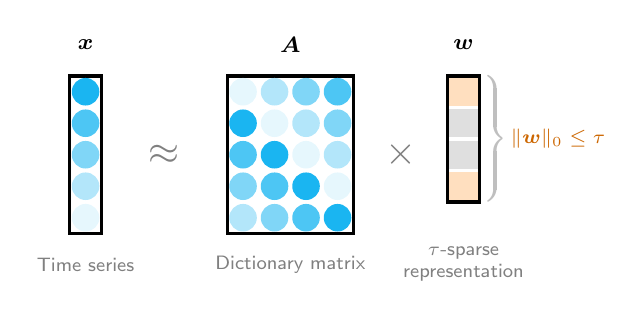
\begin{tikzpicture}[domain=0:4]
    \newcommand{\posx}{4}
    \newcommand{\posy}{3.8}

    \draw [step=0.4, very thick, color=white] (0+0.8,0-4) grid (0.4+0.8,2-4);
    \draw [very thick] (0+0.8,0-4) rectangle (0.4+0.8,2-4);
    \draw (1,3-4-0.6) node {\footnotesize{\color{black}$\boldsymbol{x}$}};
    \node[circle,fill=cyan!90,inner sep=0pt,minimum size=0.35cm] at (1,1.8-4) {};
    \node[circle,fill=cyan!70,inner sep=0pt,minimum size=0.35cm] at (1,1.4-4) {};
    \node[circle,fill=cyan!50,inner sep=0pt,minimum size=0.35cm] at (1,1-4) {};
    \node[circle,fill=cyan!30,inner sep=0pt,minimum size=0.35cm] at (1,0.6-4) {};
    \node[circle,fill=cyan!10,inner sep=0pt,minimum size=0.35cm] at (1,0.2-4) {};

    \draw (2,-3) node {\Large{\color{gray}$\approx$}};

    \draw [step=0.4, very thick, color=white] (2.8,0-4) grid (4.4,2-4);
    \draw [very thick] (2.8,0-4) rectangle (4.4,2-4);
    \draw (3.6,3-4-0.6) node {\footnotesize{\color{black}$\boldsymbol{A}$}};
    \node[circle,fill=cyan!10,inner sep=0pt,minimum size=0.35cm] at (3,1.8-4) {};
    \node[circle,fill=cyan!90,inner sep=0pt,minimum size=0.35cm] at (3,1.4-4) {};
    \node[circle,fill=cyan!70,inner sep=0pt,minimum size=0.35cm] at (3,1-4) {};
    \node[circle,fill=cyan!50,inner sep=0pt,minimum size=0.35cm] at (3,0.6-4) {};
    \node[circle,fill=cyan!30,inner sep=0pt,minimum size=0.35cm] at (3,0.2-4) {};

    \node[circle,fill=cyan!30,inner sep=0pt,minimum size=0.35cm] at (3.4,1.8-4) {};
    \node[circle,fill=cyan!10,inner sep=0pt,minimum size=0.35cm] at (3.4,1.4-4) {};
    \node[circle,fill=cyan!90,inner sep=0pt,minimum size=0.35cm] at (3.4,1-4) {};
    \node[circle,fill=cyan!70,inner sep=0pt,minimum size=0.35cm] at (3.4,0.6-4) {};
    \node[circle,fill=cyan!50,inner sep=0pt,minimum size=0.35cm] at (3.4,0.2-4) {};

    \node[circle,fill=cyan!50,inner sep=0pt,minimum size=0.35cm] at (3.8,1.8-4) {};
    \node[circle,fill=cyan!30,inner sep=0pt,minimum size=0.35cm] at (3.8,1.4-4) {};
    \node[circle,fill=cyan!10,inner sep=0pt,minimum size=0.35cm] at (3.8,1-4) {};
    \node[circle,fill=cyan!90,inner sep=0pt,minimum size=0.35cm] at (3.8,0.6-4) {};
    \node[circle,fill=cyan!70,inner sep=0pt,minimum size=0.35cm] at (3.8,0.2-4) {};

    \node[circle,fill=cyan!70,inner sep=0pt,minimum size=0.35cm] at (4.2,1.8-4) {};
    \node[circle,fill=cyan!50,inner sep=0pt,minimum size=0.35cm] at (4.2,1.4-4) {};
    \node[circle,fill=cyan!30,inner sep=0pt,minimum size=0.35cm] at (4.2,1-4) {};
    \node[circle,fill=cyan!10,inner sep=0pt,minimum size=0.35cm] at (4.2,0.6-4) {};
    \node[circle,fill=cyan!90,inner sep=0pt,minimum size=0.35cm] at (4.2,0.2-4) {};

    \draw (5,-3) node {\Large{\color{gray}$\times$}};
    
    \filldraw [fill=orange!25] (5.2+0.4,0.4-4) rectangle (5.6+0.4,2-4);
    \filldraw [fill=gray!25] (5.2+0.4,0.8-4) rectangle (5.6+0.4,1.6-4);
    \draw [step=0.4, very thick, color=white] (5.2+0.4,0.4-4) grid (5.6+0.4,2-4);
    \draw [very thick] (5.2+0.4,0.4-4) rectangle (5.6+0.4,2-4);
    \draw (5.8,3-4-0.6) node {\footnotesize{\color{black}$\boldsymbol{w}$}};

    \draw (6.2,-2.8) node[rotate = 90] {{\color{gray!50}$\underbrace{\hspace{1.6cm}}$}};
    \draw (7,-2.8) node {\scriptsize{\color{orange!80!black}$\|\boldsymbol{w}\|_0\leq\tau$}};

    \draw (1,-4.4) node {\scriptsize{\color{gray}Time series}};
    \draw (3.6,-4.4) node {\scriptsize{\color{gray}Dictionary matrix}};
    \draw (5.8,-4.25) node {\scriptsize{\color{gray}$\tau$-sparse}};
    \draw (5.8,-4.5) node {\scriptsize{\color{gray}representation}};

\end{tikzpicture}

\end{document}